
\section{Sources Detected by \Actitle{LAT}}
\seclabel{sources_detected_fermi} 

\begin{figure}[htbp]
  \centering
    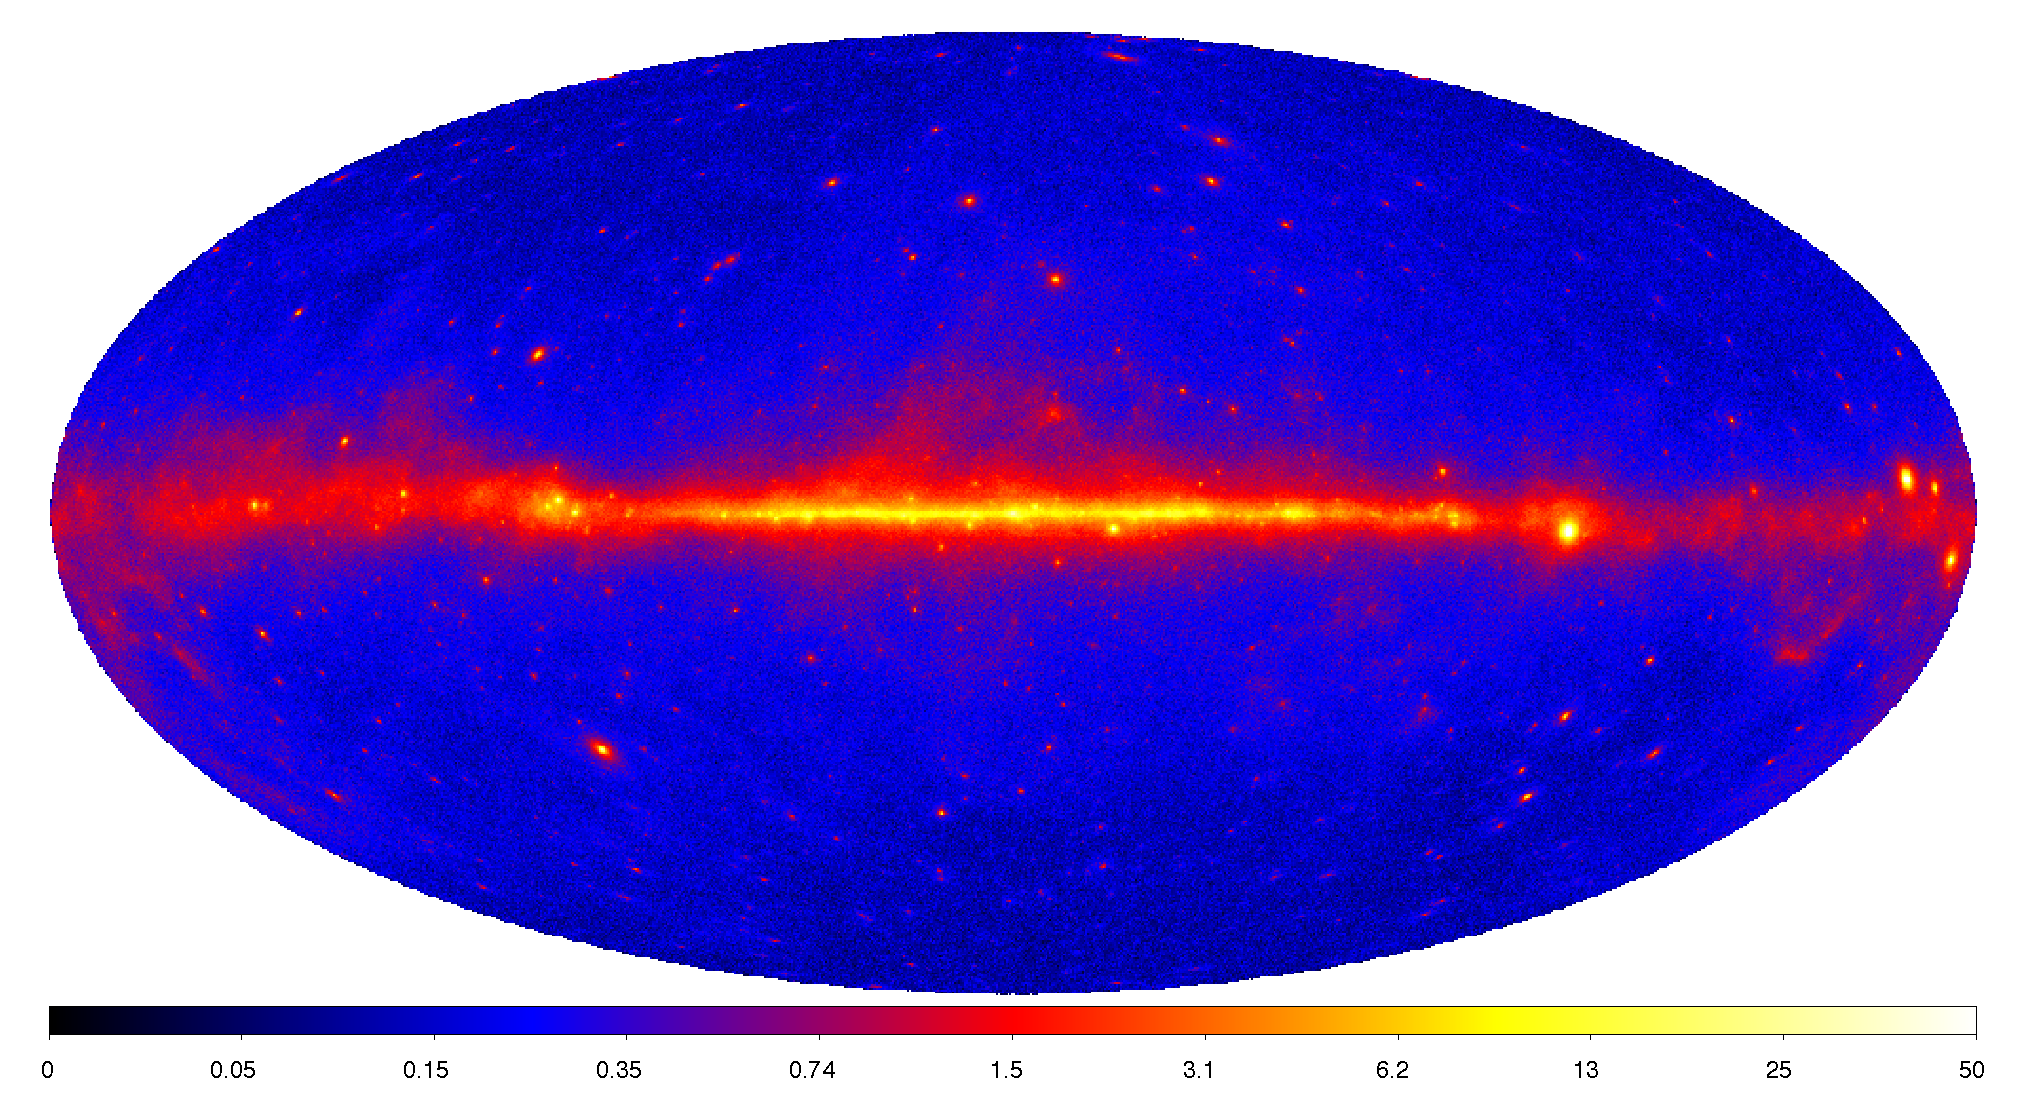
\includegraphics[width=\textwidth]{chapters/introduction/figures/lat_skymap_2fgl.pdf}
  \caption{
  An Aitoff projection map of the $\gamma$-ray sky observed by the
  \ac{LAT} with a 2 years exposure.  This map is integrated in the
  energy range from $100\unitspace\mev$ to $10\unitspace\gev$ in units
  of $10^{-7}\erg\unitspace\cm^{-2}\second^{-1}\steradian^{-1}$.  This figure is
  from \cite{nolan_2012_fermi-large}.
  }
  \figlabel{lat_skymap_2fgl}
\end{figure}

\figref{lat_skymap_2fgl} shows a map of the $\gamma$-ray sky observed
with two years of data. From this map, one can clearly observed a
strongly-structured anisotropic component of the $\gamma$-ray emission
from the galaxy. In addition, many individual sources of $\gamma$-rays
can be viewed. In \subsecref{galactic_diffuse_and_isotropic}, we
discuss the Galactic diffuse and isotropic $\gamma$-ray background. In
\subsecref{2fgl}, we discuss \ac{2FGL}, a catalog of point-like
sources detected by the \ac{LAT}. In \subsecref{2pc}, we discuss
\ac{2PC}, a catalog of pulsars detected by the \ac{LAT}.  Finally,
in \subsecref{pwn_detected_lat} we discuss \acp{PWN} detected by the
\ac{LAT}.


\subsection{The Galactic Diffuse and Isotropic Gamma-ray Background}
\subseclabel{galactic_diffuse_and_isotropic}

the interaction of cosmic-ray electrons and protons with the gas in our
Milky Way (through the \pion and bremsstrahlung process) and with the
Galactic radiation fiels (through the \ac{IC} process).

Much work has gone into theoreically moding the diffuse
$\gamma$-ray emission. The most advanced theoretical model
of Galactic emission from or galaxy comes from the \galprop code
\citep{strong_1998a_propagation-cosmic-ray,moskalenko_2000a_anisotropic-inverse}.
In addition, significant work by \cite{abdo_2009a_fermi-large} and
\cite{ackermann_2012a_fermi-lat-observations} have gone into comparing
these theoreitcal predictions to the observed $\gamma$-ray intensity
distrubtions observed by the \ac{LAT}.

In addition to an anisotropic Galactic diffuse background, the \ac{LAT}
observes an isotropic component to the $\gamma$-ray distribution.
This emission is believed to be a composite of unresolved extragalactic
point-like sources as well as a residual charged-particle background.
\cite{abdo_2010a_spectrum-isotropic} presenets detailed measurements of
isotropic background observed by the \ac{LAT}.

The \galprop predictions for the $\gamma$-ray background are not
accurate enough for the analysis of point-like (and $\sim1\degree$
large extended sources).  Therefore, an improved data-driven model
of the Galactic diffuse background has been devised where components
of the \galprop model are fit to the observed $\gamma$-ray emission.
This data-driven model is described in \cite{nolan_2012_fermi-large}.


\subsection{\Actitle{2FGL}}
\subseclabel{2fgl}

\Ac{2FGL} was a catalog by the \ac{LAT} collaboration containing XXX Sources.
\todo[inline]{Describe Catalog}

\begin{itemize}
  \item Citation is \cite{nolan_2012_fermi-large}
  \item Source classification method
  \item Number of sources detected by the \ac{LAT}
  \item Forward reference \chapref{maximum_likelihood_analysis},
    which does a more thorough description of likelihood analysis method.
  \item Source classes/associations
\end{itemize}

\subsection{\Actitle{2PC}}
\subseclabel{2pc}

\Ac{2PC} is a \ldots
\seclabel{second_pulsar_catalog}

\begin{itemize}
  \item Process of detecting Pulsars with the \ac{LAT}
  \item Number of pulsars detected by the \ac{LAT}
\end{itemize}

\subsection{\Acptitle{PWN} Detected by \Actitle{LAT}}
\subseclabel{pwn_detected_lat}

\subsubsection{Crab}

\subsubsection{Vela X}

\subsubsection{MSH 15-52}

\todo[inline]{Dig up HESS reference of HESS J1514-59.}

\subsubsection{\hessj{1825}}

\hessj{1825} is a cool source

HESS Detection: 
HESS Energy dependent morphology: \cite{aharonian_2006a_energy-dependent}

LAT Detection: \cite{grondin_2011_detection-pulsar}



\subsubsection{\hessj{1640}}

\hessj{1640} is also cool.

HESS detection:  \cite{aharonian_2006a_h.e.s.s.-survey}
Fermi detection: \cite{slane_2010_fermi-detection}

\subsubsection{\hessj{1857}}

\hessj{1857} is another good source.

LAT detection: \cite{rousseau_2012_fermi-lat-constraints}

\begin{enumerate}
  \item \url{http://arxiv.org/pdf/1206.3324v1.pdf}
\end{enumerate}

\subsubsection{J1023}

\ldots
